\documentclass{article}

\usepackage{graphicx}
\usepackage{tikz}
\usepackage{tikzsymbols}
\usetikzlibrary{calc,patterns,shapes.geometric}
\pagestyle{empty}
\usepackage[margin=0pt]{geometry}
\geometry{papersize={14in,12in}}

\def\centerarc[#1](#2)(#3:#4:#5){\draw[#1] ($(#2)+({#5*cos(#3)},{#5*sin(#3)})$) arc (#3:#4:#5);}

\begin{document}
	\begin{figure}
		\centering
		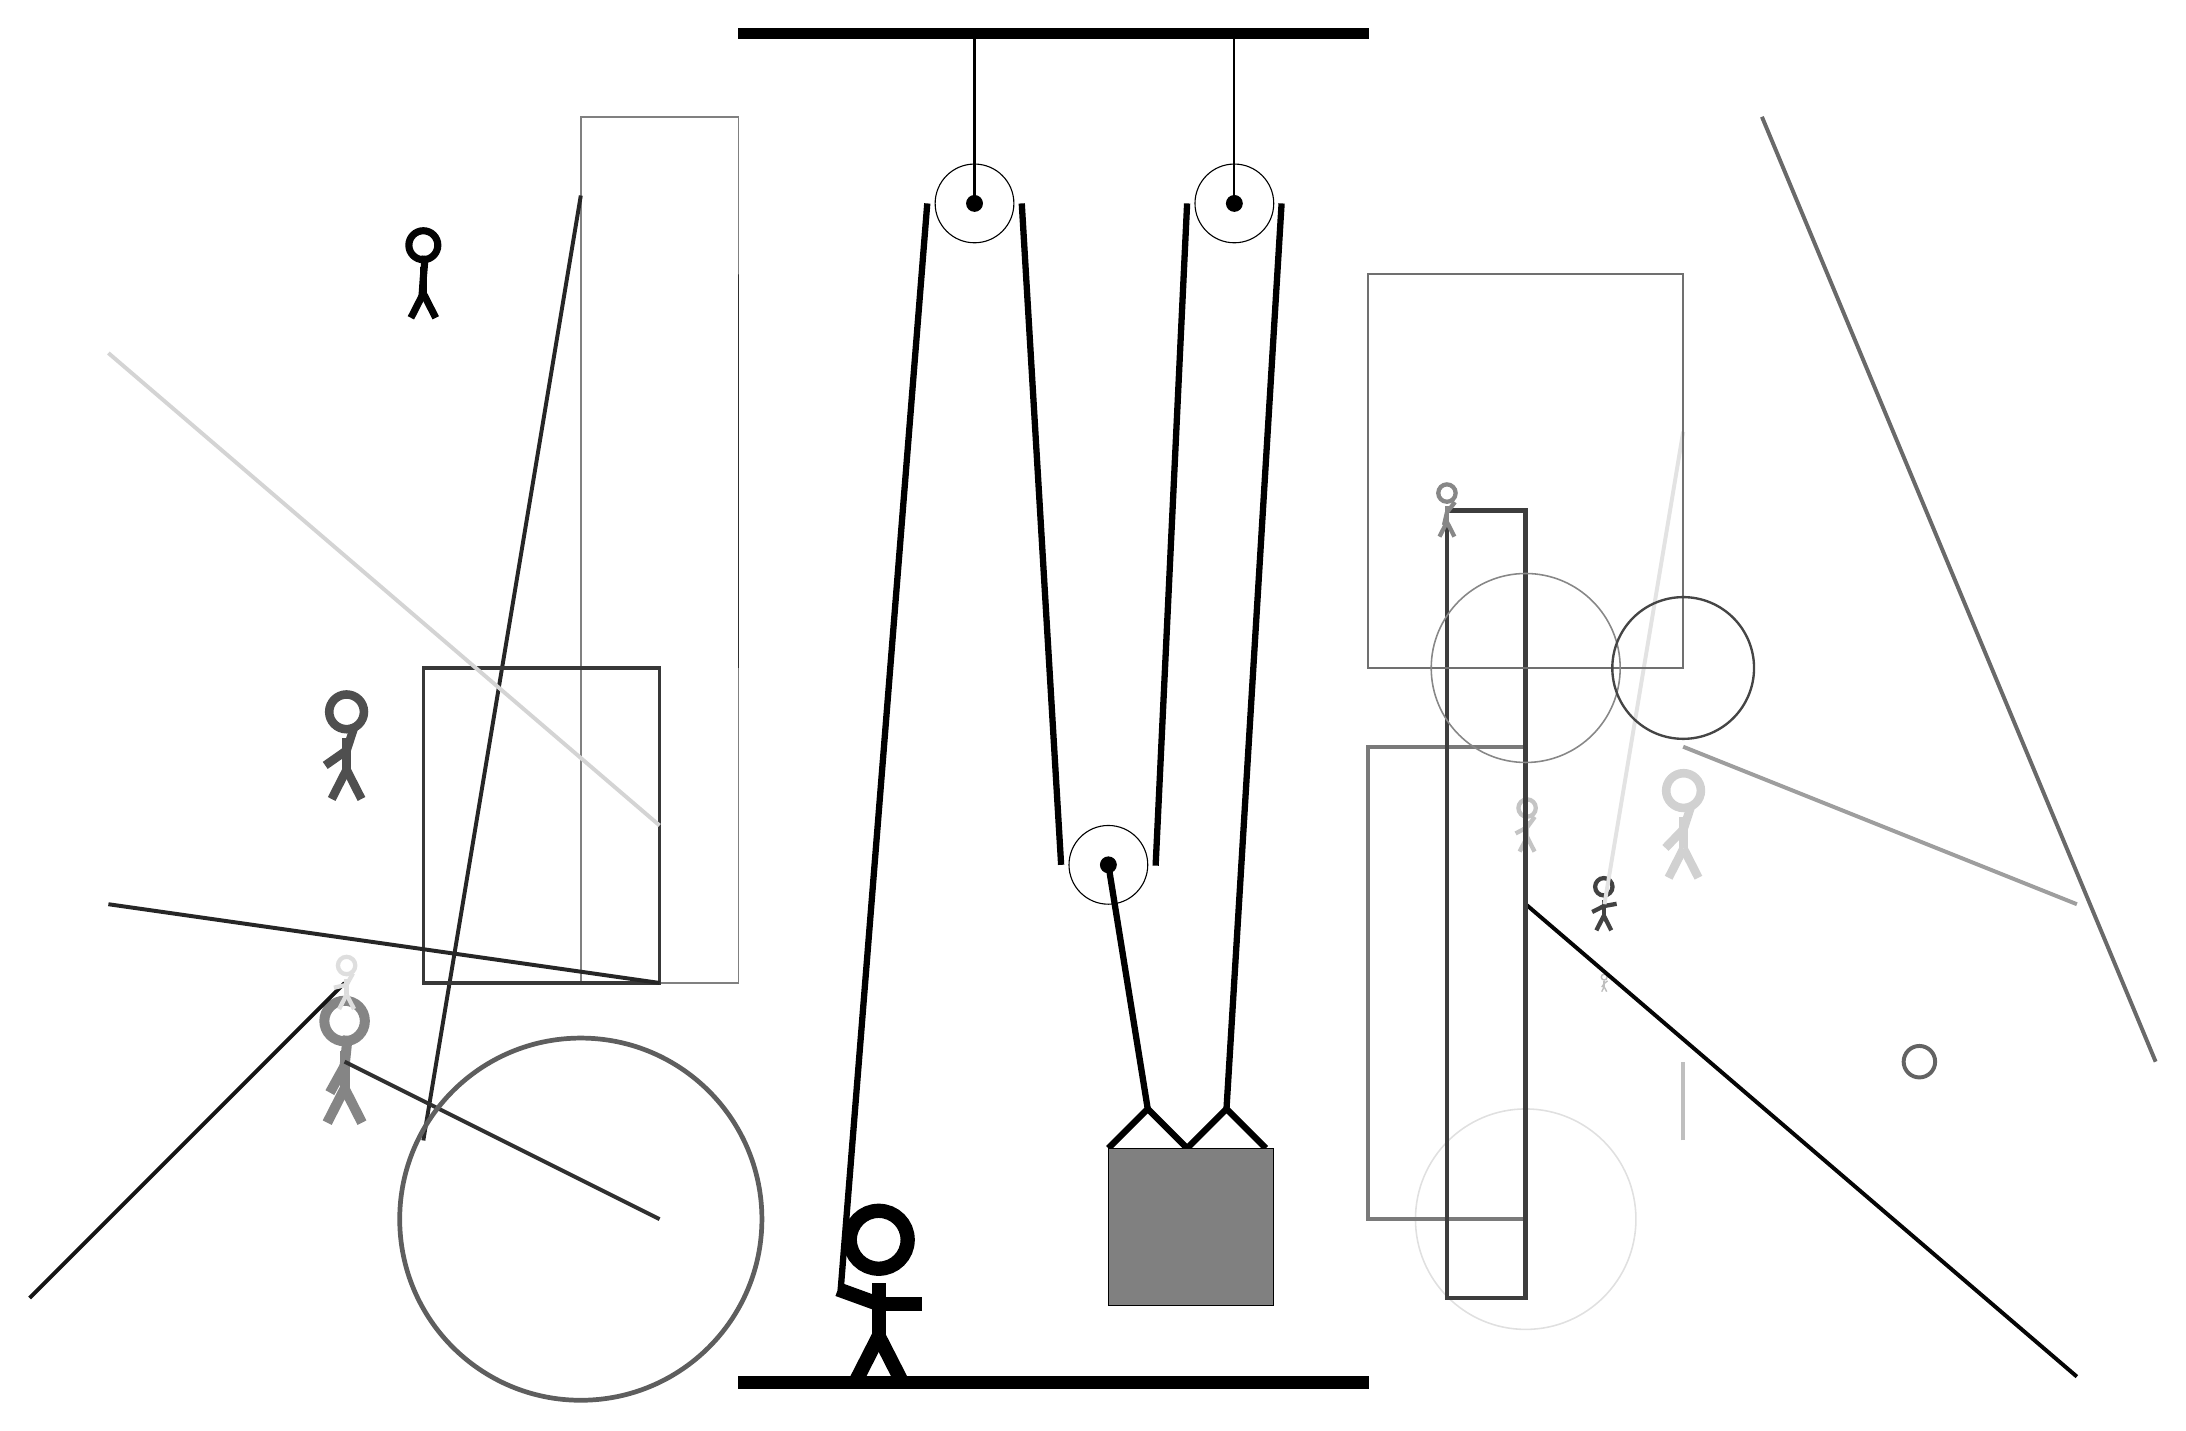
\begin{tikzpicture}
			%%%%% START %%%%%
			
			\draw[fill=black] (-2, 14) rectangle (6, 14.125);
			
			\draw (1, 11.9) circle (0.5);
			\draw[fill=black] (1, 11.9) circle (0.1);
			\draw[thick] (1, 11.9) -- (1, 14);
			
			\draw (4.3, 11.9) circle (0.5);
			\draw[fill=black] (4.3, 11.9) circle (0.1);
			\draw[thick] (4.3, 11.9) -- (4.3, 14);
			
			\draw (2.7, 3.5) circle (0.5);
			\draw[fill=black] (2.7, 3.5) circle (0.1);
			
			\draw[line width=0.8mm]  (2.7, -0.1) -- (3.2, 0.4) -- (3.7, -0.1) -- (4.2, 0.4) -- (4.7, -0.1);
			\draw[fill=black!50] (2.7, -0.1) rectangle (4.8, -2.1);
			
			\draw[line width=0.8mm](-0.7, -1.9) -- (0.4, 11.9);
			\centerarc[line width=0.8mm](1, 11.9)(0:180:0.6);
			\draw[line width=0.8mm](1.6, 11.9) -- (2.1, 3.5);
			\centerarc[line width=0.8mm](2.7, 3.5)(180:370:0.6);
			\draw[line width=0.8mm] (3.3, 3.49) -- (3.7, 11.9);
			\centerarc[line width=0.8mm](4.3, 11.9)(0:180:0.6);
			\draw[line width=0.8mm](4.2, 0.4) -- (4.9, 11.9);
			\draw[line width=0.8mm] (3.2, 0.4) -- (2.7, 3.5);
			
			\node[line width=0.7mm, color=black!74] at (9, 3) {\Strichmaxerl[3][27][10]};
			
			\draw[line width=0.5mm, color=black!59](11, 13) -- (16, 1);
			\node[line width=0.4mm, color=black!48] at (-7, 1) {\Strichmaxerl[7][61][84]};
			\node[line width=0.7mm, color=black!18] at (10, 4) {\Strichmaxerl[6][46][72]};
			\node[line width=0.7mm, color=black!99] at (-6, 11) {\Strichmaxerl[5][86][85]};
			
			\draw [line width=0.6mm, color=black!10](8, 5) circle (0.0);
			\node[line width=0.5mm, color=black!25] at (9, 2) {\Strichmaxerl[1][56][39]};
			\node[line width=0.7mm, color=black!23] at (8, 4) {\Strichmaxerl[3][28][54]};
			\draw [line width=0.2mm, color=black!12](8, -1) circle (1.4);
			\draw[line width=0.5mm, color=black!98](8, 3) -- (15, -3);
			
			\draw [line width=0.5mm, color=black!61](13, 1) circle (0.2);
			\draw[line width=0.2mm, color=black!50] (-4, 2) rectangle (-2, 13);
			\draw[line width=0.5mm, color=black!52] (6, 5) rectangle (8, -1);
			\node[line width=0.7mm, color=black!69] at (-7, 5) {\Strichmaxerl[6][35][72]};
			\draw[line width=0.5mm, color=black!92](-7, 2) -- (-11, -2);
			\draw[line width=0.5mm, color=black!85](-6, 0) -- (-4, 12);
			\draw[line width=0.6mm, color=black!76] (7, -2) rectangle (8, 8);
			\draw[line width=0.2mm, color=black!82] (-2, 6) rectangle (-2, 11);
			\draw[line width=0.4mm, color=black!78] (-3, 2) rectangle (-6, 6);
			\node[line width=0.4mm, color=black!47] at (7, 8) {\Strichmaxerl[3][77][52]};
			\draw[line width=0.5mm, color=black!38](10, 5) -- (15, 3);
			
			\draw[line width=0.5mm, color=black!11](9, 3) -- (10, 9);
			\draw[line width=0.5mm, color=black!25](10, 0) -- (10, 1);
			\draw[line width=0.5mm, color=black!81](-7, 1) -- (-3, -1);
			\draw[line width=0.2mm, color=black!56] (6, 6) rectangle (10, 11);
			
			\draw [line width=0.6mm, color=black!63](-4, -1) circle (2.3);
			\node[line width=0.5mm, color=black!13] at (-7, 2) {\Strichmaxerl[3][13][61]};
			\draw [line width=0.2mm, color=black!47](8, 6) circle (1.2);
			
			\draw [line width=0.3mm, color=black!73](10, 6) circle (0.9);
			
			\draw[line width=0.5mm, color=black!85](-3, 2) -- (-10, 3);
			\draw[line width=0.5mm, color=black!17](-3, 4) -- (-10, 10);
			
			
			\node at (-0.2, -2) {\Strichmaxerl[10][-20][0]};
			
			\draw[fill=black] (-2, -3) rectangle (6, -3.15);
			
			%%%%% END %%%%%
		\end{tikzpicture}
	\end{figure}	
\end{document}